\documentclass[12pt, letterpaper]{article}

\usepackage{amsmath}
\usepackage{graphicx}

% set path to images
\graphicspath{{./images/}}

% load persian language and select font
\usepackage{xepersian}
\settextfont{BNazanin}

\title{گزارش کار پروژه اول آنالیز عددی 1}
\author{گروه 6}

\begin{document}
\maketitle

\section{سوال 1}
\subsection{صورت سوال}
فرض کنید \(fl(y)\) عدد \(k\) رقمی قطع شده \(y\) باشد، نشان دهید:

\[\frac{\big| y-fl(y) \big| }{\big| y \big|} \le 10^{-k+}\]

\subsection{پاسخ}

% answer to question 1


% leave space between question 1 and 2
\vspace{5mm}

% start of question 2
\section{سوال 2}
\subsection{صورت سوال}
فرض کنید
\(f(x) = \frac{2 \cdot log(1+x) \: + \: 2 \cdot i tan^{-1}(ix) \: + \: x^2}{-x^4}\)
و 
\(\lim_{x\to 0}\frac{f(x)}{x^p} = C \ne 0\)
با داشتن سری مکلورن توابع 
\(log(x)\)
و 
\(tan^{-1}(x)\)
مقادیر 
\(C\)
و 
\(p\)
را بیابید.

\subsection{پاسخ}
همانطور که در فایل میپل حل این سوال قابل مشاهده است، در مرحله اول با تعریف ظابطه اصلی تابع و رسم نمودار آن سعی میکنیم درکی هندسی از رفتار آن بیابیم. نمودار اول نشان میدهد که تابع در 0 به مقداری نزدیک به 0 میل میکند. اما با برسی دقیق تر و محدود کردن دامنه نمایش نمودار مشاهده میشود که تابع در مقادیر نزدیک به صفر شدیدا نوسان میکند. \\
% insert the 2 plot of f(x) 

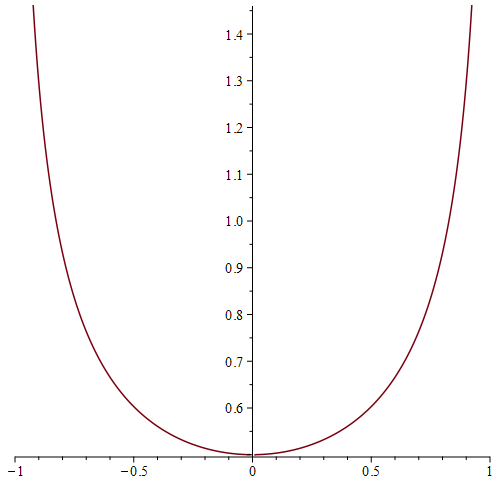
\includegraphics[height=5cm, width=7cm]{figure1.png}
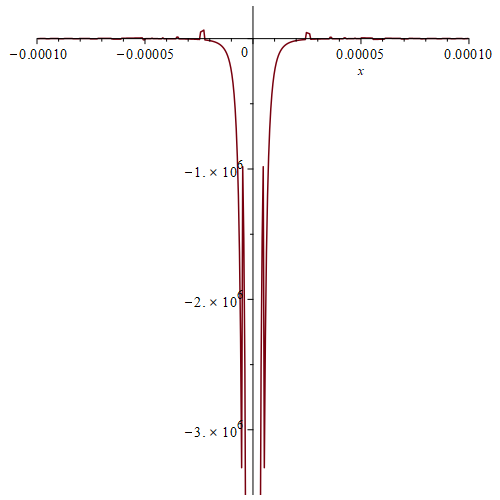
\includegraphics[height=5cm, width=7cm]{figure2.png}
\\


برای حل سوال در ابتدا بسط مکلورن توابع را تا درجه 10 محاسبه میکنیم. نرم افزار میپل از
\(O(x^y)\)
 برای نمایش درجه خطا در یک سری تیلور استفاده میکند. یا این توصیف با افزایش تعداد جملات سری تیلور یا درجه آن میتوان خطا را تا حد توانایی مجاسباتی کامپیوتر کاهش داد. اما چون در این مورد 
\(x\)
 بسیار نزدیک به 0 است میتوان با همین درجه پیش رفت چرا که وقتی 
\(x\) 
 نزدیک به صفر است 
\(x^{11}\)
 بسیار کوچک خواهد بود.
\\

\end{document}























